\apendice{Especificación de diseño}

\section{Introducción}

En esta sección se describe cómo están implementados los datos de esta aplicación, cuáles son los procedimientos más relevantes y cómo se organizan los proyectos.

\section{Diseño de datos}

En esta sección, explicaremos como están organizados tanto el conjunto de imágenes obtenidas, cómo son y como se organizan las características extraídas de las imágenes, y el diagrama de clases de la aplicación.

\subsection{Conjunto de imágenes}

El conjunto de imágenes es el descrito en \cite{GDXray:imagenes}. Estas imágenes están disponibles en un repositorio público: \url{https://drive.google.com/drive/folders/143893UAlc7TB_ZiTGlg9S9w4rp3wHlji}. Este repositorio contiene 5 grupos de carpetas una para cada grupo: \textit{Castings}, \textit{Welds}, \textit{Baggage}, \textit{Nature} y \textit{Settings}. Estas imágenes son almacenadas en formato de escala de grises de 8 bits ``png'' (\textit{Portable Network Graphics}). También tenemos metadatos adicionales para cada serie en un archivo ASCII llamado Xssss\_readme.txt incluido en la subcarpeta Xssss, donde ``X'' es la inicial del grupo y ``ssss'' es el número de serie del grupo de imágenes. Para este proyecto sólo hemos utilizado el grupo \textit{Castings}.

En \cite{GDXray:imagenes} este grupo se describe como: ``(...)contiene 2.727 imágenes de rayos-x organizadas en 67 series. Las imágenes de rayos-x se tomaron principalmente de partes automotrices (ruedas de aluminio y nudillos) usando un intensificador de imágenes. (...)Es interesante resaltar que la serie C0001 contiene no solo una secuencia de 72 imágenes de rayos-x tomadas de una rueda de aluminio girando su eje central, pero también anotaciones de \textit{Bounding Boxes} de la verdad del terreno (\textit{ground truth}) de 226 pequeños defectos y la matriz de calibración de cada imagen que relaciona las coordenadas 3D de la rueda de aluminio con coordenadas 2D de la imagen de rayos-x'' (p.4-p.5).

\subsection{Diagrama de clases de la aplicación}

En este apartado se comentará las clases realizadas por nosotros en el proyecto. Es decir, las clases que se han creado para realizar la aplicación. Señalamos que, únicamente se analizaran las realizadas por nosotros, toda la estructura del repositorio \texttt{metal-defect-detection} \cite{metal-defect-detection:repositorio} no será analizada.

\subsubsection{Clases de la aplicación}

Para la aplicación se han creado las siguientes clases:

\begin{itemize}
    \item \texttt{XrayDataset} dentro de \texttt{app.py}: Clase que contiene el conjunto de datos de las imágenes de rayos-X, tiene una sola función que crea un conjunto de datos compuesto por una imagen con su id, su directorio, su altura y su anchura también crean una clase ``\textit{Casting Defect}'' que es el tipo de defectos que puede haber.
    \item \texttt{Detector} dentro de \texttt{app.py}: Clase que contiene toda la estructura gráfica de la ventada de la aplicación. Se inicializan todos los elementos gráficos (\textit{frames}, botones...), las variables necesarias para cada uno, y los mediadores. También contiene todos los métodos necesarios para la visualización de las imágenes, la detección de los defectos y la visualización de las máscaras y la información adicional de los defectos. Debido a que todo se encuentra en la misma clase la mayoría de funciones no devuelve nada.
    \item \texttt{InferenceConfig} dentro de \texttt{app.py}: Clase que contiene únicamente dos variables para la configuración del \texttt{config}. Esta configuración hace que se ejecute la detección de defectos en una solo imagen cada vez.
\end{itemize}

\imagen{diagrama_clases}{Diagrama de clases}

\section{Diseño procedimental}

\subsection{Diagramas de secuencia}

En este apartado se mostrarán los diagramas de secuencia respectivos a 4 tareas de la aplicación:

\begin{itemize}
    \item Cargar de imágenes, ver figura \ref{DS_carga}.
    \item Predecir los defectos de las imágenes y mostrar la imagen con los defectos, ver figura \ref{DS_predecir}.
    \item Visualizar la información de los defectos, ver figura \ref{DS_info}.
    \item Visualizar las máscaras de los defectos, ver figura \ref{DS_masks}.
\end{itemize}

\newpage

\begin{figure}[H]
	\centering
	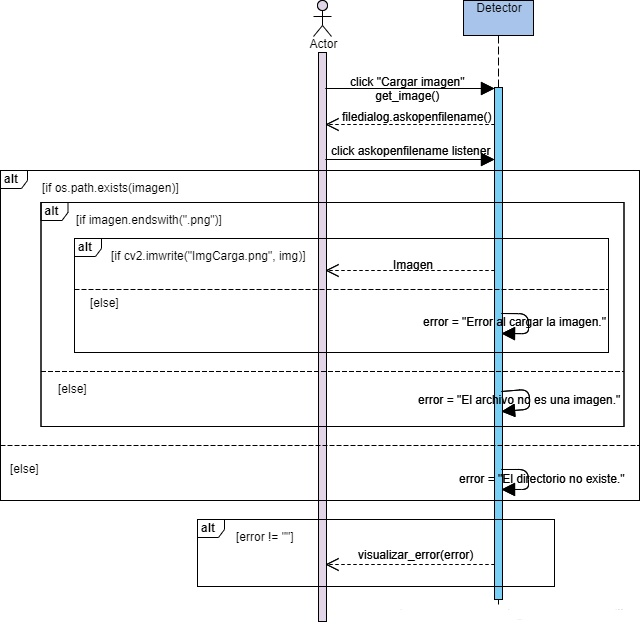
\includegraphics[scale=0.7]{DS_carga}
	\caption{Diagrama de secuencia para la cargar una imagen}
	\label{DS_carga}
\end{figure}

\begin{figure}[H]
	\centering
	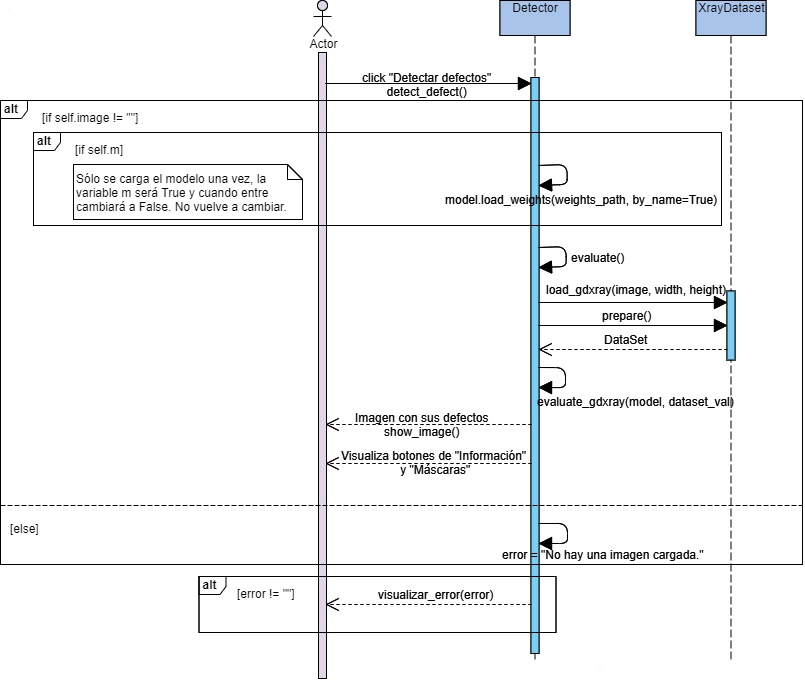
\includegraphics[scale=0.6]{DS_predecir}
	\caption{Diagrama de secuencia para la predicción y muestra de defectos}
	\label{DS_predecir}
\end{figure}

\begin{figure}[H]
	\centering
	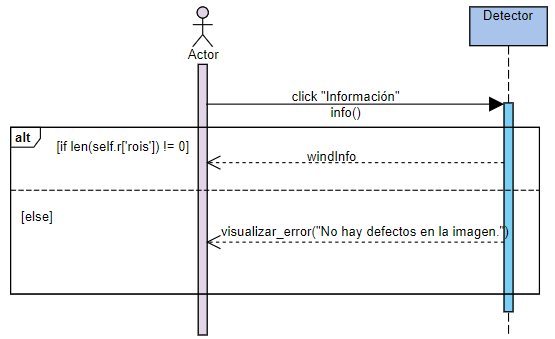
\includegraphics[scale=0.9]{DS_info}
	\caption{Diagrama de secuencia para la muestra de la información de los defectos}
	\label{DS_info}
\end{figure}

\begin{figure}[H]
	\centering
	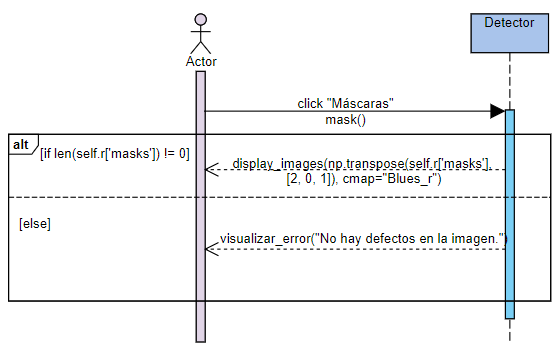
\includegraphics[scale=0.9]{DS_masks}
	\caption{Diagrama de secuencia para la muestra de las máscaras de los defectos}
	\label{DS_masks}
\end{figure}

\section{Diseño arquitectónico}

En este apartado se definirá el diseño arquitectónico de la aplicación, la cual sigue el patrón de diseño \textit{Singleton}.

\subsection{Patrón Singleton}

El patrón de diseño \textit{Singleton} \cite{singleton} (instancia única) está diseñado para restringir la creación de objetos pertenecientes a una clase o el valor de un tipo a un único objeto. Su intención consiste en garantizar que una clase sólo tenga una instancia y proporcionar un punto de acceso global a ella. No se encarga de la creación de objetos en sí, sino que se enfoca en la restricción en la creación de un objeto.